%%%%%%%%%%%%%%%%%%%%%%%%%%%%%%%%%%%%%%%%%%%%%%%%%%%%%%%%%%%%%%%%%%%%%%%%%%%%%%%%%%%%%%%
%%%%%%%%%%%%%%%%%%%%%%%%%%%%%%%%%%%%%%%%%%%%%%%%%%%%%%%%%%%%%%%%%%%%%%%%%%%%%%%%%%%%%%%
% 
% This top part of the document is called the 'preamble'.  Modify it with caution!
%
% The real document starts below where it says 'The main document starts here'.

\documentclass[12pt]{article}

\usepackage{amssymb,amsmath,amsthm}
\usepackage[top=1in, bottom=1in, left=1.25in, right=1.25in]{geometry}
\usepackage{fancyhdr}
\usepackage{graphicx}
\usepackage{enumerate}
\usepackage{verbatim}
\usepackage{listings}
\usepackage{xcolor}

% Comment the following line to use TeX's default font of Computer Modern.
\usepackage{times,txfonts}

\definecolor{codegreen}{rgb}{0,0.6,0}
\definecolor{codegray}{rgb}{0.5,0.5,0.5}
\definecolor{codepurple}{rgb}{0.58,0,0.82}
\definecolor{backcolour}{rgb}{0.95,0.95,0.92}

\lstdefinestyle{mystyle}{
    backgroundcolor=\color{backcolour},   
    commentstyle=\color{codegreen},
    keywordstyle=\color{magenta},
    numberstyle=\tiny\color{codegray},
    stringstyle=\color{codepurple},
    basicstyle=\ttfamily\footnotesize,
    breakatwhitespace=false,         
    breaklines=true,                 
    captionpos=b,                    
    keepspaces=true,                 
    numbers=left,                    
    numbersep=5pt,                  
    showspaces=false,                
    showstringspaces=false,
    showtabs=false,                  
    tabsize=2
}

\lstset{style=mystyle}

\newtheoremstyle{homework}% name of the style to be used
  {18pt}% measure of space to leave above the theorem. E.g.: 3pt
  {12pt}% measure of space to leave below the theorem. E.g.: 3pt
  {}% name of font to use in the body of the theorem
  {}% measure of space to indent
  {\bfseries}% name of head font
  {:}% punctuation between head and body
  {2ex}% space after theorem head; " " = normal interword space
  {}% Manually specify head
\theoremstyle{homework} 

% Set up an Exercise environment and a Solution label.
\newtheorem*{exercisecore}{\@currentlabel}
\newenvironment{exercise}[1]
{\def\@currentlabel{#1}\exercisecore}
{\endexercisecore}

\newcommand{\localhead}[1]{\par\smallskip\noindent\textbf{#1}\nobreak\\}%
\newcommand\solution{\localhead{Solution:}}



% \newcommand{includematlab}[1]{\verbatiminput{#1}}

%%%%%%%%%%%%%%%%%%%%%%%%%%%%%%%%%%%%%%%%%%%%%%%%%%%%%%%%%%%%%%%%%%%%%%%%
%
% Stuff for getting the name/document date/title across the header
\makeatletter
\RequirePackage{fancyhdr}
\pagestyle{fancy}
\fancyfoot[C]{\ifnum \value{page} > 1\relax\thepage\fi}
\fancyhead[L]{\ifx\@doclabel\@empty\else\@doclabel\fi}
\fancyhead[C]{\ifx\@docdate\@empty\else\@docdate\fi}
\fancyhead[R]{\ifx\@docauthor\@empty\else\@docauthor\fi}
\headheight 15pt

\def\doclabel#1{\gdef\@doclabel{#1}}
\doclabel{Use {\tt\textbackslash doclabel\{MY LABEL\}}.}
\def\docdate#1{\gdef\@docdate{#1}}
\docdate{Use {\tt\textbackslash docdate\{MY DATE\}}.}
\def\docauthor#1{\gdef\@docauthor{#1}}
\docauthor{Use {\tt\textbackslash docauthor\{MY NAME\}}.}
\makeatother

%% General formatting parameters
\parindent 0pt
\parskip 12pt plus 1pt

\def\vx{\mathbf x}
\def\vb{\mathbf b}

% Shortcuts for blackboard bold number sets (reals, integers, etc.)
\newcommand{\Reals}{\ensuremath{\mathbb R}}
\newcommand{\Nats}{\ensuremath{\mathbb N}}
\newcommand{\Ints}{\ensuremath{\mathbb Z}}
\newcommand{\Rats}{\ensuremath{\mathbb Q}}
\newcommand{\Cplx}{\ensuremath{\mathbb C}}
%% Some equivalents that some people may prefer.
\let\RR\Reals
\let\NN\Nats
\let\II\Ints
\let\CC\Cplx

%%%%%%%%%%%%%%%%%%%%%%%%%%%%%%%%%%%%%%%%%%%%%%%%%%%%%%%%%%%%%%%%%%%%%%%%%%%%%%%%%%%%%%%
%%%%%%%%%%%%%%%%%%%%%%%%%%%%%%%%%%%%%%%%%%%%%%%%%%%%%%%%%%%%%%%%%%%%%%%%%%%%%%%%%%%%%%%
% 
% The main document start here.

% The following commands set up the material that appears in the header.

%%%%%%%%%%%%%%%%%%%%%%%%%%%%%%%%%%%%%%%%%%%%%%%%%%%%%%%%%%%%%%%%%%%%%%%%%%
\doclabel{Math 426: Homework 12}
\docauthor{Andrew Player}
\docdate{November 18, 2020}

\begin{document}


\begin{exercise}{Text 8.10}
\end{exercise}
\begin{verbatim}
Polynomials:
  2a_0(0)  + b0 = 0
  a_0(0)^2 + b_0(0) + c_0 = 1
  a_0(1)^2 + b_0(1) + c_0 = 2
  a_1(1)^2 + b_1(1) + c_1 = 2
  a_1(2)^2 + b_1(2) + b_1 = 0
  a_2(2)^2 + b_2(2) + b_2 = 0
  2a_0(0) + b_1 - 2a_2(0) - b_2 = 0
  2a_1(1) + b_1 - 2a_2(1) - b_2 = 0
  a_1 = 0
\end{verbatim}


\begin{exercise}{Text 8.12}
\end{exercise}
\begin{verbatim}
The pins have the correct output values:
  1+(0)-(0)^3 = 1 
  1 - 2(1-1)-3(1-1)^2+4(1-1)^3 = 1
  4(2-2)+9(2-2)^2-3(2-2)^3 = 0
  4(3-2)+9(3-2)^2-3(3-2)^3 = 10

The spline is twice continuosly differentiable:
  s' (x) = { 1-3x^2        | if 0 <= x <  1
           { 2(8-15x+6x^2) | if 1 <= x <  2
           { -68+54x-9x^2  | if 2 <= x <= 3
  
  s''(x) = { -6x           | if 0 <= x <  1
           { 6(4x-5)       | if 1 <= x <  2
           { -18(x-3)      | if 2 <= x <= 3

  Continuity Check:
    1-,1+: 1-3(1)^2          == 2(8-15(1)+6(1)^2) Good
    2-,2+: 2(8-15(2)+6(2)^2) == -68+54(2)-9(2)^2  Good

    1-,1+: -6(1)     == 6(4(1)-5) Good
    2-,2+: 6(4(2)-5) == -18(2-3)  Good

Since the spline is cubic, has the correct output values,
and is twice continously differentiable at each of the pins,
it is a natural cubic spline. 
\end{verbatim}

\begin{exercise}{Text 8.13}
\end{exercise}
\begin{verbatim}
1-,1+:
------------------------
0th Derivative:
  ax^2+b(x-1)^3 = cx^2+d
  a = c + d
1st Derivative:
  2ax+3b(x-1)^2 = 2cx
  2a = 2c
  a = c
2nd Derivative:
  2a+6b(x-1) = 2c
  2a = 2c
  a = c

2-,2+
------------------------
0th Derivative:
  cx^2+d = ex^2+(x-2)^3
  4c + d = 4e
1st Derivative:
  2cx = 2ex+3b(x-2)^2
  2c = 2e
  c = e
2nd Derivative: 
  2c = 2e+6b(x-2)
  2c = 2e
  c = e

So, when a = c = e, b = f = 0, and d is
and real number, it is a cubic spline.  
\end{verbatim}

\begin{exercise}{Text 8.14}
\end{exercise}
Code:
\begin{lstlisting} [language=Matlab]
>> x  = linspace(0, 1, 21);
>> xx = linspace(0, 1);
>> y  = exp(-2*x).*sin(10*pi*x);
>> s  = spline(x, y);
>> yi = ppval(s, xx)
\end{lstlisting}
Plot:\newline
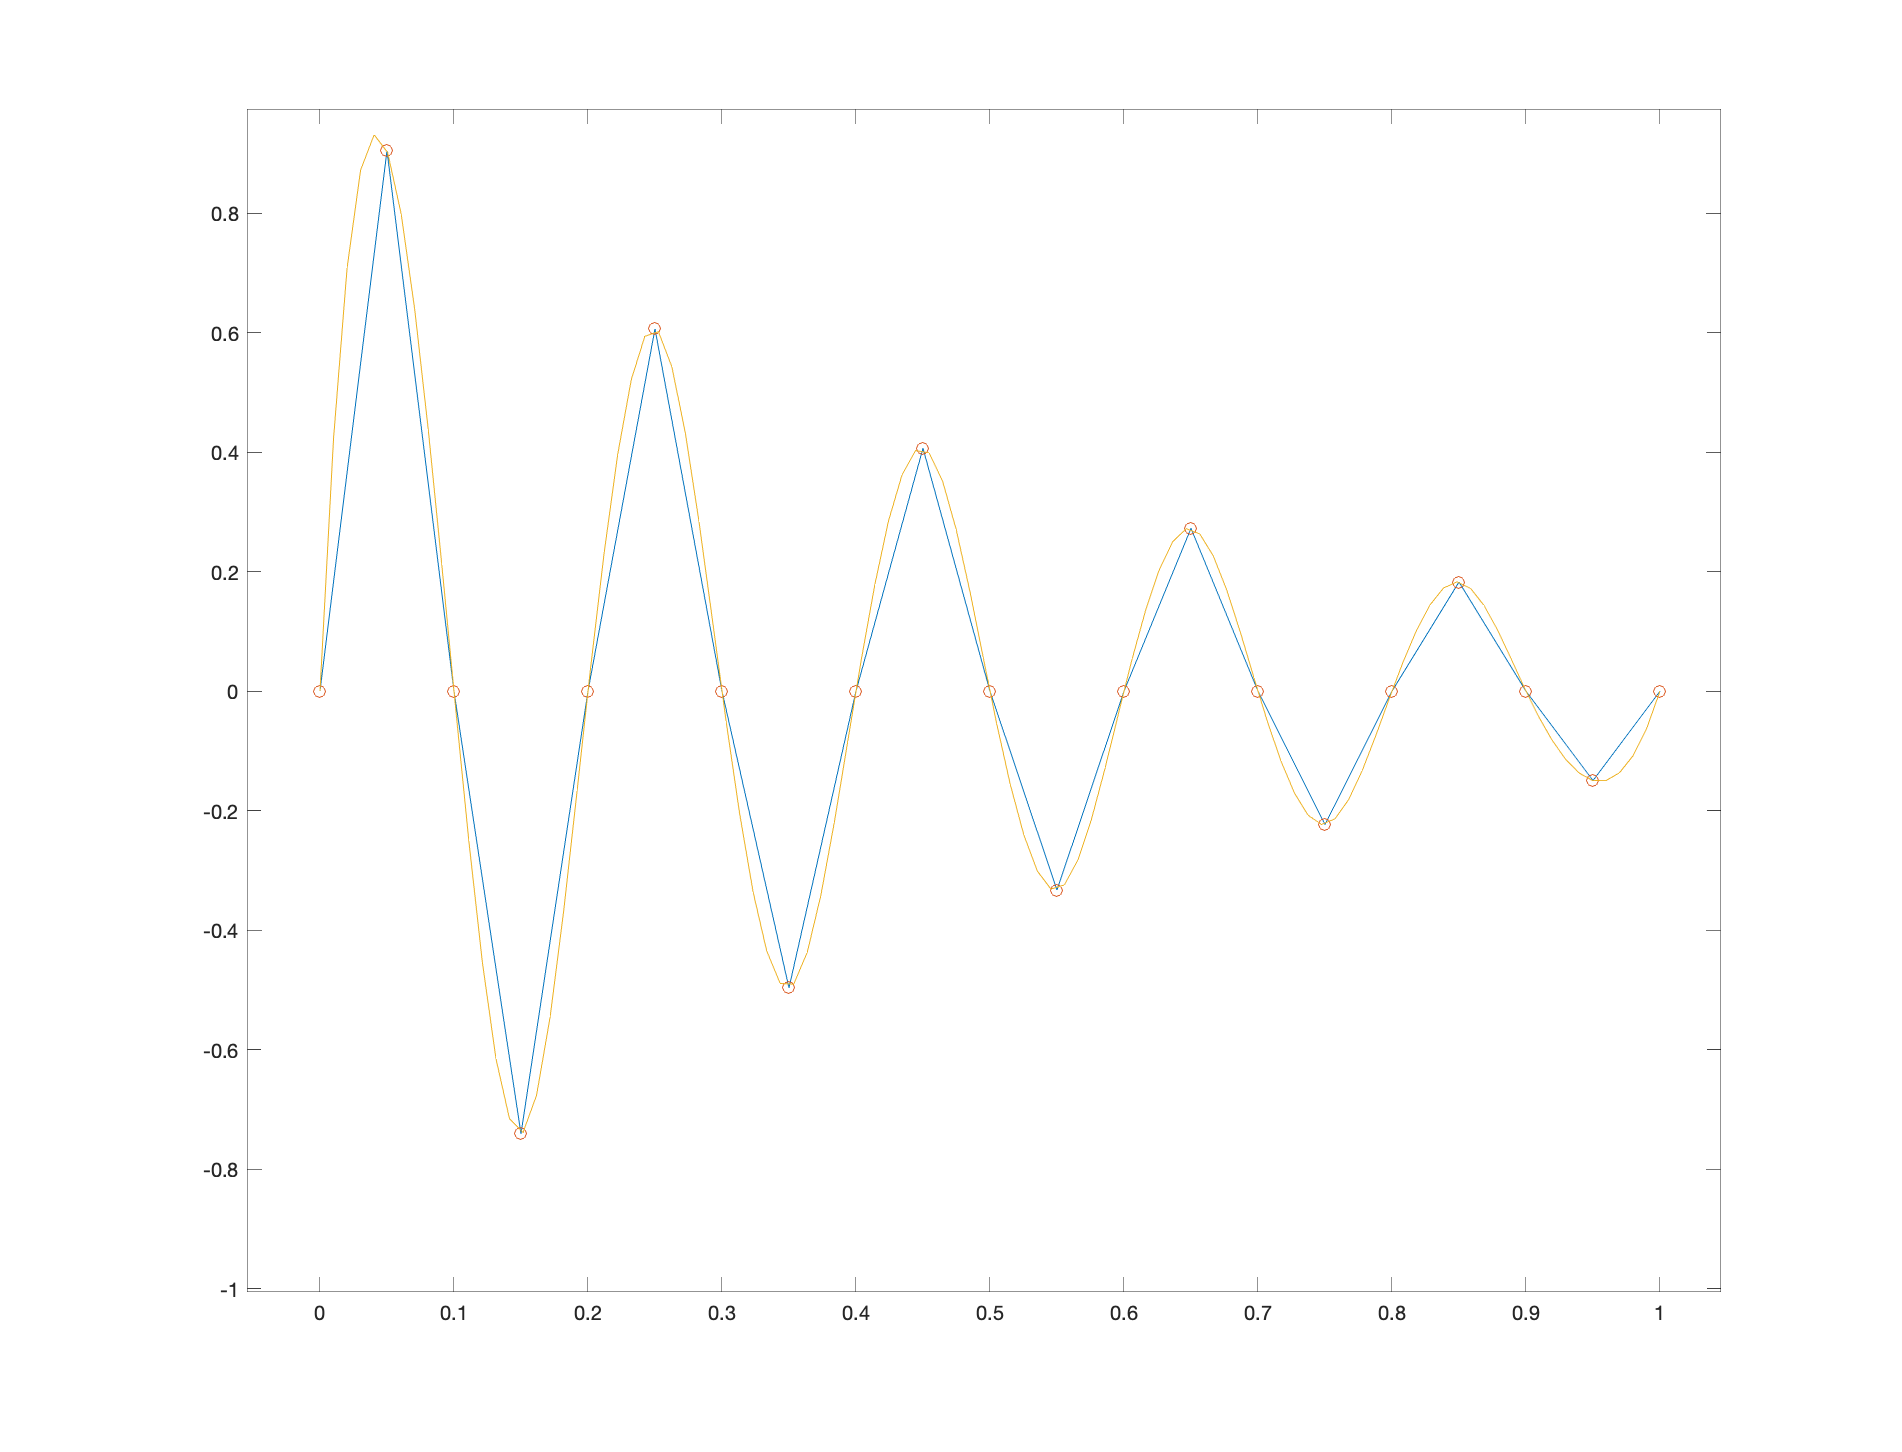
\includegraphics[scale=0.2]{8_14.png}


\begin{exercise}{Text 10.1}
\end{exercise}
B:
$\begin{bmatrix}
1 & 1 & 1 \\
x_{1}&x_{2}&x_{3}&x^{4} \\
x^{2}_{1}&x^{2}_{2}&x^{2}_{3}&x^{2}_{4} \\
x^{3}_{1}&x^{3}_{2}&x^{3}_{3}&x^{3}_{4}
\end{bmatrix}$\newline
b:
$\begin{bmatrix}
b-a \\
\frac{b^{2}}{2} - \frac{a^{2}}{2} \\
\frac{b^{3}}{3} - \frac{a^{3}}{3} \\
\frac{b^{4}}{4} - \frac{a^{4}}{4}
\end{bmatrix}$ \newline
A = x -> Bx = b\newline
A = x = $\begin{bmatrix}
\frac{1}{8} \\
\frac{3}{8} \\
\frac{3}{8} \\
\frac{1}{8}
\end{bmatrix}$\newline
So, $\frac{1}{8}f(0)+\frac{3}{8}f(\frac{1}{3})+\frac{3}{8}f(\frac{2}{3})+\frac{1}{8}f(1)$
\begin{exercise}{Text 10.2}
\end{exercise}
Integral$ = ae^{1}-a+\frac{2b}{\pi}$\newline
        $ = \frac{2b}{(a+b)\pi}(a+b) + 1(ae)$\newline
Where, $A0 = \frac{2b}{(a+b)\pi}$, $A1 = 1$
and  , $f(0) = (a+b)$, $f(1) = (ae)$
\end{document}